\documentclass[a4paper, 12pt]{article}
\usepackage{polski}
\usepackage[utf8]{inputenc}
\usepackage{listings}
\usepackage{graphicx}
\author{Marcin Fabrykowski}
\title{Modelowanie procesów fizycznych\\Laboratorium 1}
\begin{document}

\lstset{
  literate={ą}{{a}}1
           {ó}{{o}}1
           {ł}{{l}}1
           {ę}{{e}}1
           {ć}{{c}}1
}
\maketitle
\newpage
\section{Kod programu}
\lstinputlisting[language=Python]{lab01.py}
\section{Obserwacja uzyskanych trajektorii}
Pięć losowych trajektorii zostało zaprezentowanych na rys. \ref{fig:tr1}, \ref{fig:tr2}, \ref{fig:tr3}, \ref{fig:tr4}, \ref{fig:tr5}.
\begin{figure}[h]
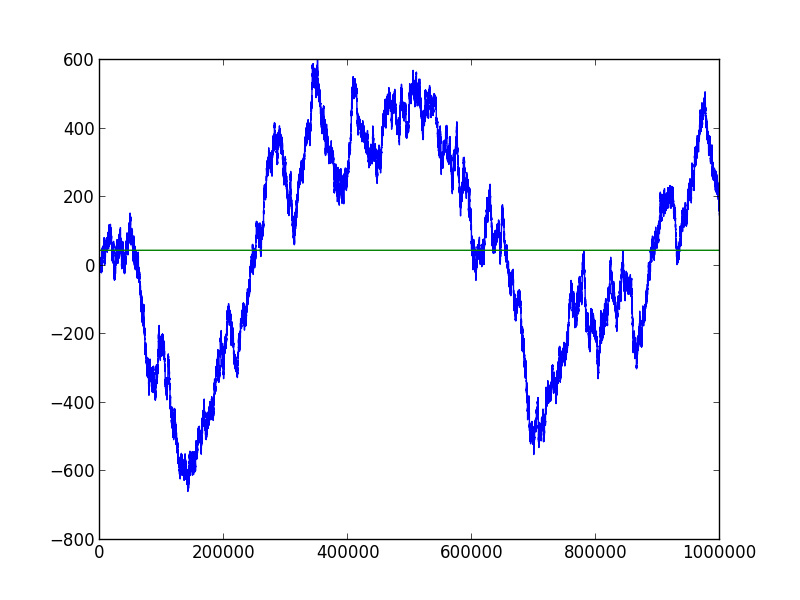
\includegraphics[scale=0.5]{traj1.png}
\caption{Trajektoria}
\label{fig:tr1}
\end{figure}
\begin{figure}[h]
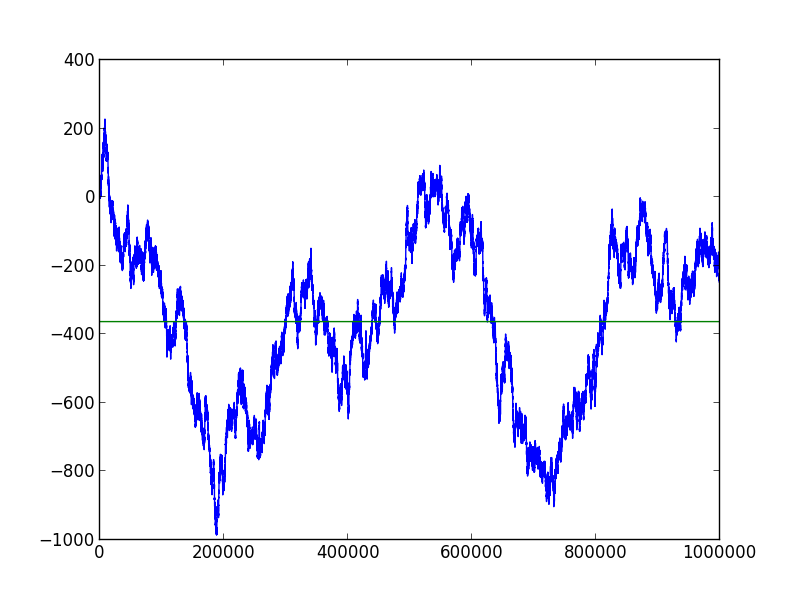
\includegraphics[scale=0.5]{traj2.png}
\caption{Trajektoria}
\label{fig:tr2}
\end{figure}
\begin{figure}[h]
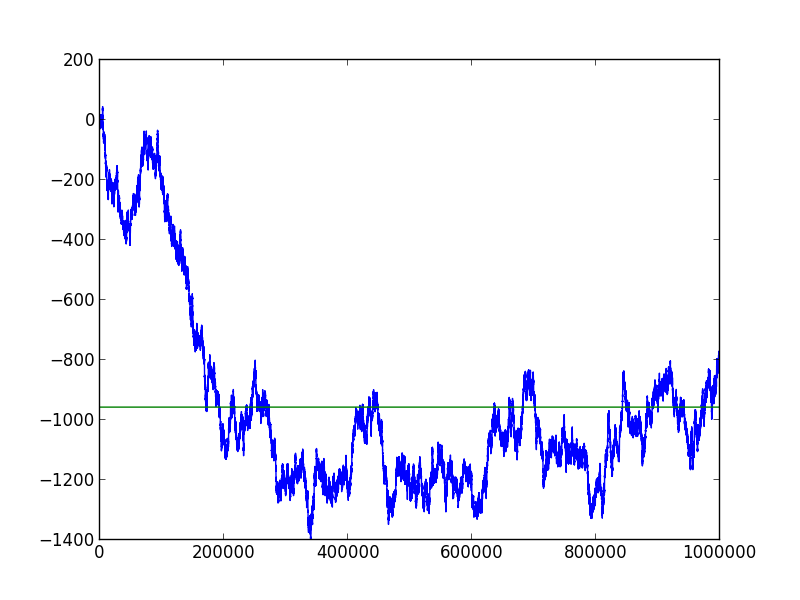
\includegraphics[scale=0.5]{traj3.png}
\caption{Trajektoria}
\label{fig:tr3}
\end{figure}
\begin{figure}[h]
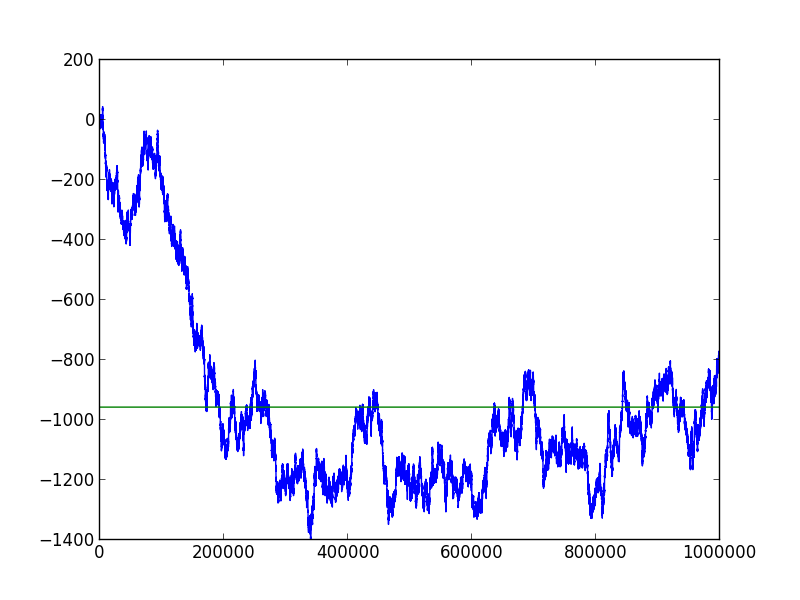
\includegraphics[scale=0.5]{traj3.png}
\caption{Trajektoria}
\label{fig:tr4}
\end{figure}
\begin{figure}[h]
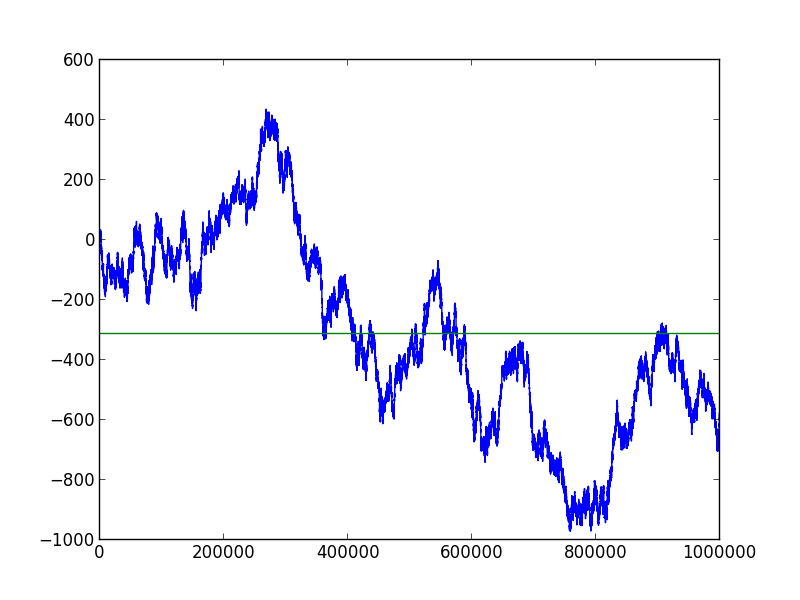
\includegraphics[scale=0.5]{traj5.png}
\caption{Trajektoria}
\label{fig:tr5}
\end{figure}
\section{Obserwacja własności samo podobieństwa}
Na rys. \ref{fig:kor1}, \ref{fig:kor10}, \ref{fig:kor1000}, przedstawiono graficzną reprezentację autokorelacji z przesunięciami odpowiednio 1, 10 oraz 1000.
\begin{figure}[h]
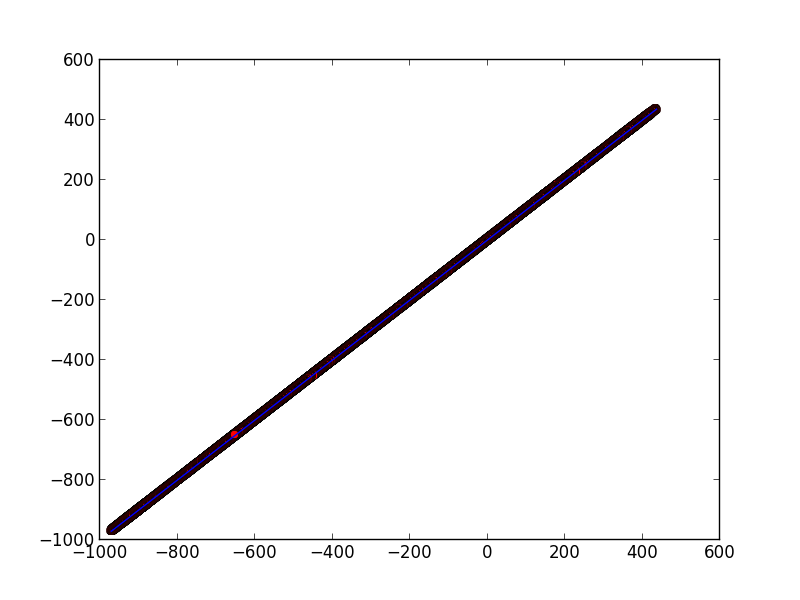
\includegraphics[scale=0.5]{out1.png}
\caption{Autokorelacja, przesunięcie 1}
\label{fig:kor1}
\end{figure}
\begin{figure}[h]
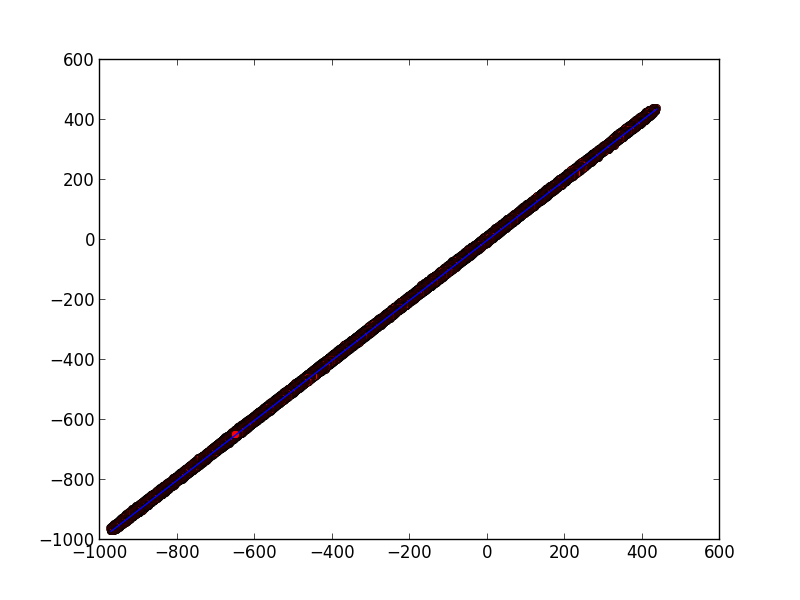
\includegraphics[scale=0.5]{out10.png}
\caption{Autokorelacja, przesunięcie 10}
\label{fig:kor10}
\end{figure}
\begin{figure}[h]
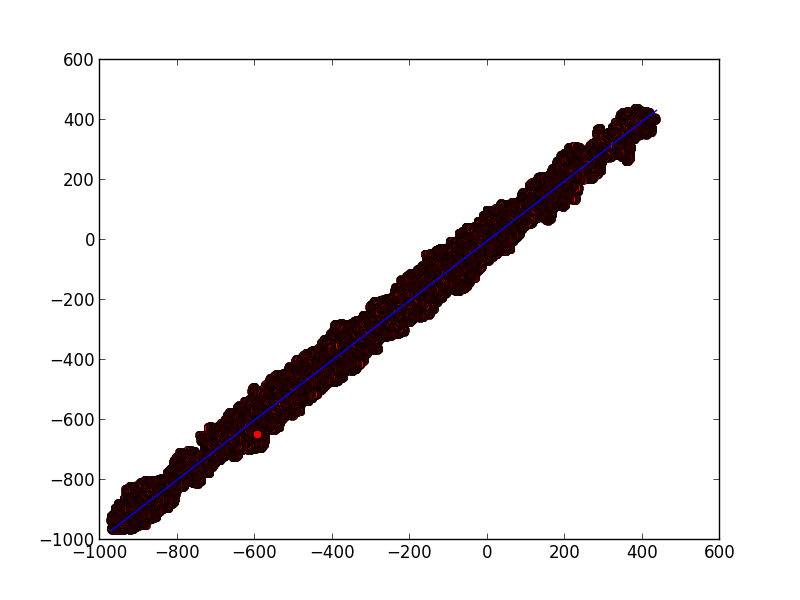
\includegraphics[scale=0.5]{out1000.png}
\caption{Autokorelacja, przesunięcie 1000}
\label{fig:kor1000}
\end{figure}
\end{document}
